\section{Vektoren}
\subsection{Definition von Vektoren}
\begin{defi}{Vektoren}{}\index{Vektoren!Definition}
Die Menge aller parallelen, gleich langen und gleich gerichteten Pfeile nennt man Vektor. Jeder Pfeil ist der Repräsentant des Vektors.
\begin{center}

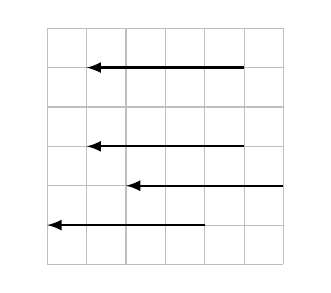
\begin{tikzpicture}[x=.5cm, y=.5cm,domain=-9:9,smooth, cross/.style={draw, cross out,
  minimum size=2*(#1-1pt), inner sep=0pt, outer sep=0pt},>=latex, font= \footnotesize]
   %Raster zeichnen
   \draw [color=gray!50]  [step=5mm] (-1,-1) grid (5,5);

\coordinate(a) at (4,4);
\coordinate(b) at (0,4);

\coordinate(c) at (4,2);
\coordinate(d) at (0,2);

\coordinate(e) at (5,1);
\coordinate(f) at (1,1);

\coordinate(g) at (3,0);
\coordinate(h) at (-1,0);
%Vektor
\draw[thick, ->] (a) node[right]{} -- (b) node[left]{};
\draw[thick, ->] (c) node[right]{} -- (d) node[left]{};
\draw[thick, ->] (e) node[right]{} -- (f) node[left]{};
\draw[thick, ->] (g) node[right]{} -- (h) node[left]{};
\end{tikzpicture}
\end{center}
Alle drei Pfeile sind Repräsentanten des selben Vektors.
\end{defi}
\begin{merke}{Bezeichnungen}{}\index{Vektoren!Bezeichnung}
Vektoren werden mit kleinen lateinischen Buchstaben und einem pfeil gekennzeichnet $\vec{u}$. Verläuft ein Repräsentant eines Vektors von einem Punkt z.B. $P$ zu einem zweiten Punkt z.B. $Q$, so bezeichnet man alle Repräsentanten mit $\vv{PQ}$.
\begin{center}

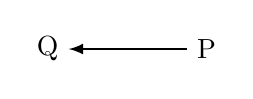
\begin{tikzpicture}[x=.5cm, y=.5cm,domain=-9:9,smooth, cross/.style={draw, cross out,
  minimum size=2*(#1-1pt), inner sep=0pt, outer sep=0pt},>=latex, ]
   %Raster zeichnen
% \draw [color=gray!50]  [step=5mm] (0,0) grid (3,3);
\coordinate(a) at (3,3);
\coordinate(b) at (0,3);
%Vektor
\draw[thick, ->] (a) node[right]{P} -- (b) node[left]{Q};
\end{tikzpicture}
\end{center}
\end{merke}
\begin{satz}{Vektoraddition}{}\phantomsection\label{vekadd}\index{Vektoren!Addition}
Bei der Addition von zwei Vektoren wird an den Endpunkt eines Repräsentanten des ersten Vektors $\vv{a}$ der Beginn eines Repräsentanten des zweiten Vektors $\vv{b}$ gesetzt. Der Pfeil des Summenvektors $\vv{c} = \vv{a} + \vv{b}$ ergibt sich durch den Pfeil der am Anfangspunkt des Vektors $\vv{a}$ beginnt und am Endpunkt des Vektors $\vv{b}$ endet.\\
Da es für einen Vektor unendlich viele Repräsentanten gibt, gibt es immer einen, der an der \glqq richtigen\grqq{} Stelle für eine Addition liegt.
\begin{center}
 
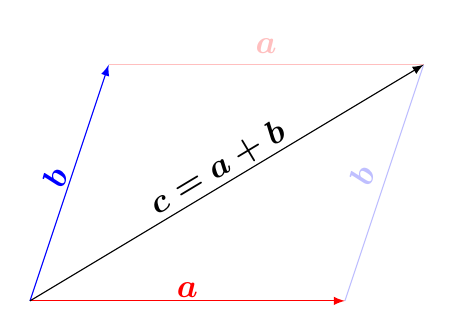
\begin{tikzpicture}[font=\boldmath]\large
    % Punkte
    \coordinate (A) at (0,0) {};
    \coordinate (B) at (4,0) {};
    \coordinate (C) at (1,3) {};
    \coordinate (D) at (5,3) {};

    % Draw the triangle
    \draw[blue!25]  (B) -- (D) node[sloped,midway,above] {$\vv{b}$};
    \draw[red!25]   (C) -- (D) node[sloped,midway,above] {$\vv{a}$};;
    \draw[->,  red,   arrows={-latex}]  (A) -- (B) node[sloped,midway,above=-0.1cm] {$\vv{a}$};
    \draw[->,  blue,  arrows={-latex}]  (A) -- (C) node[sloped,midway,above=-0.1cm] {$\vv{b}$};
    \draw[->, black, arrows={-latex}]  (A) -- (D) node[sloped,midway,above=-0.1cm] {$\vv{c} = \vv{a} + \vv{b} $};
\end{tikzpicture}
\end{center}
\end{satz}
\begin{satz}{Kommutativgesetz der Vektoraddition}{}\phantomsection\label{komuvekadd}
  Wie aus der Zeichnung bei Satz \ref{vekadd} leicht ersichtlich ist, ist die Addition von Vektoren kommutativ. Es gilt also: $$\vv{a} + \vv{b} = \vv{b} +\vv{a}$$ 
\end{satz}
\begin{satz}{Kommutativgesetz der Vektoraddition}{}
  Wie aus der Zeichnung bei Satz \ref{vekadd} leicht ersichtlich ist, ist die Addition von Vektoren kommutativ. Es gilt also: $$\vv{a} + \vv{b} = \vv{b} +\vv{a}$$ 
\end{satz}

\begin{satz}{Assoziativgesetz der Vektoraddition}{}\phantomsection\label{assivekadd}
\begin{center}
 Bei der Addition von Vektoren gilt das Assoziativgesetz. Es gilt also:
 $$(\vv{a} + \vv{b}) + \vv{c} = \vv{a} + (\vv{b} + \vv{c}) = \vv{a} + \vv{b} +\vv{c}$$
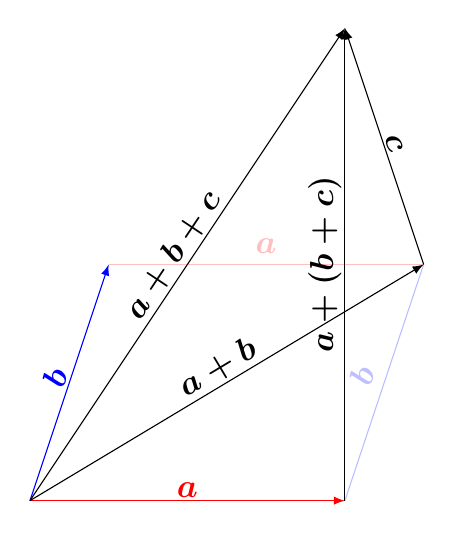
\begin{tikzpicture}[font=\boldmath]\large
    % Punkte
    \coordinate (A) at (0,0) {};
    \coordinate (B) at (4,0) {};
    \coordinate (C) at (1,3) {};
    \coordinate (D) at (5,3) {};
    \coordinate (E) at (4,6) {};

    % Draw the triangle
    \draw[blue!25]  (B) -- (D) node[sloped,midway,above] {$\vv{b}$};
    \draw[red!25]   (C) -- (D) node[sloped,midway,above] {$\vv{a}$};
    \draw[->,  red,   arrows={-latex}]  (A) -- (B) node[sloped,midway,above=-0.1cm] {$\vv{a}$};
    \draw[->,  blue,  arrows={-latex}]  (A) -- (C) node[sloped,midway,above=-0.1cm] {$\vv{b}$};
    \draw[->, black, arrows={-latex}]  (A) -- (D) node[sloped,midway,above=-0.1cm] {$ \vv{a} + \vv{b} $};
    \draw[->,  black,   arrows={-latex}]  (D) -- (E) node[sloped,midway,above=-0.1cm] {$\vv{c}$};
    \draw[->,  black,   arrows={-latex}]  (A) -- (E) node[sloped,midway,above=-0.1cm] {$\vv{a} + \vv{b} + \vv{c}$};
     \draw[->,  black,   arrows={-latex}]  (B) -- (E) node[sloped,midway,above=-0.1cm] {$\vv{a} + (\vv{b} + \vv{c})$};
\end{tikzpicture}
\end{center}
\end{satz}
\begin{b8d}{Besondere Vektoren}{}\index{Vektoren!Nullvektor}\index{Vektoren!Gegenvektor}
Bei der Rechnung mit Vektoren gibt es zwei besondere Vektoren zu betrachten. Hierbei handelt es sich um den sogenannten Nullvektor und den Gegenvektor.\\
Der Nullvektor $\vv{o}$ ist derjenige Vektor, der die Länge Null hat und bei dem sich bei er Addition mit anderen Vektoren nichts ändert. Es gilt: $$\vv{a} +\vv{o} = \vv{o} +\vv{a} = \vv{a}$$
Der Gegenvektor $-\vv{a}$ ist derjenige Vektor, der genauso lang wie der Vektor $\vv{a}$ ist allerdings entgegengerichtet. Für den Gegenvektor $-\vv{a}$ und den Vektor $\vv{a}$ gilt: $$\vv{a} +( -\vv{a} ) =\vv{a}-\vv{a}= \vv{o}$$
\end{b8d}
\begin{bem}{Vektorkette}{}\index{Vektoren!Vektorkette}
Werden mehrere Vektoren addiert so werden die jeweiligen Repräsentanten aneinandergereiht und das Ergebnis nennt man dann Vektorkette.
\end{bem}
\subsection{Vektor und Skalar}
\begin{merke}{Skalar}{}\index{Vektoren!Skalar}
   In der Analytischen Geometrie versteht man unter einem Skalar eine beliebige reelle Zahl. 
\end{merke}
\begin{defi}{Skalare Multiplikation}{}\index{Vektoren!Skalare Multiplikation}
Ein Vektor kann mit einer reellen Zahl durch eine Multiplikation verknüpft werden. Der Vektor $\lambda \cdot \vv{u}$ ist $|\lambda|$-mal so lang wie der Vektor $\vv{u}$. Dabei gilt für dis Zahl $\lambda$ folgendes $\lambda \in \mathds{R}$.\\
Für $\lambda > 0$ hat der Vektor $\lambda \cdot \vv{u}$ die gleiche Richtung wie der Vektor $\vv{u}$.\\
Für $\lambda < 0$ hat der Vektor $\lambda \cdot \vv{u}$ die entgegengesetzte Richtung wie der Vektor  $\vv{u}$.\\
\begin{center}
\begin{tikzpicture}[font=\boldmath]\large
    % Punkte
    \coordinate (A) at (0,0) {};
    \coordinate (B) at (2,1) {};
    \coordinate (C) at (6,2) {};
    \coordinate (D) at (2,0) {};
    \draw[->,  arrows={-latex}]  (A) -- (B) node[sloped,midway,above=-0.1cm] {$\vv{u}$};
    \draw[->,  arrows={-latex}]  (D) -- (C) node[sloped,midway,above=-0.1cm] {$2\cdot \vv{u}$};   
\end{tikzpicture}
\end{center}
\end{defi}
\begin{satz}{Rechenregeln für das Skalarprodukt}{}\index{Vektoren!Skalare Multiplikation}
Die Skalare Multiplikation folgt zwei Gesetzmäßigkeiten. dabei gilt $\lambda, \mu \in \mathds{R}$:
\begin{itemize}
    \item Assoziativgesetz: $\lambda \cdot \left(\mu \cdot \vv{u}\right) =\left( \mu \cdot \lambda \right)\vv{u}$
    \item Distributivgesetz 1: $\lambda \cdot \left(\vv{u} + \vv{v}\right) =\lambda \cdot \vv{u} + \lambda \cdot \vv{v} $
    \item Distributivgesetz 2: $\left( \lambda + \mu\right) \cdot \vv{u} =\lambda \cdot \vv{u} + \mu \cdot \vv{u}  $
\end{itemize}
\end{satz}
\begin{bem}{}{}
Beim aufstellen einer Vektorkette versucht man den Anfangs- und Endpunkt eines Vektors durch bekannte Vektoren zu verbinden. Der Vektor $\vv{AB}$ beginnt im Punkt $A$ und endet im Punkt $B$.

\end{bem}
\begin{bsp}{Vektorkette}{}
Die Vektoren $\vv{a}=\vv{AB}, \vv{b}=\vv{AD}$ und $\vv{c}=\vv{AS}$  spannen eine vierseitige Pyramide ABCDS auf, deren Grundfläche ein Parallelogramm ABCD ist. Der Fußpunkt der Pyramidenhöhe ist der Schnittpunkt der Diagonalen der Grundfläche.   
\begin{center}
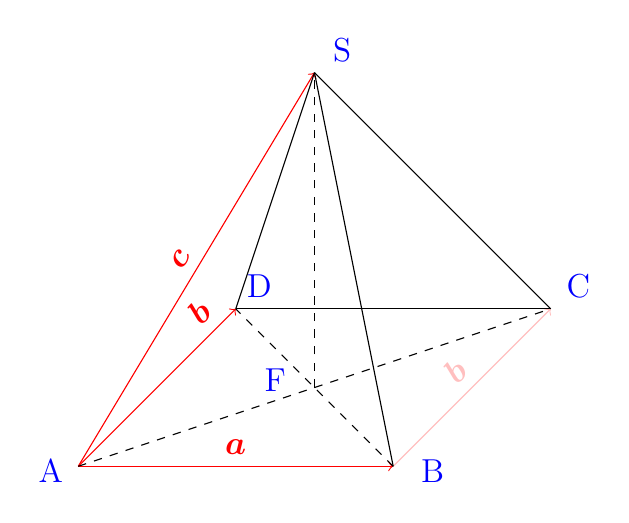
\begin{tikzpicture}[font=\boldmath]\large
    % Punkte
    \coordinate (A) at (0,0) {};
     \draw[blue] (-0.35,-0.35)   node [above] {A};
    \coordinate (B) at (4,0) {};
    \draw[blue] (4.5,-0.35)   node [above] {B};
    \coordinate (C) at (6,2) {};
    \draw[blue] (6.35,2)   node [above] {C};
    \coordinate (D) at (2,2) {};
    \draw[blue] (2.3,2)   node [above] {D};
    \coordinate (E) at (3,5) {};
    \draw[blue] (3.35,5)   node [above] {S};
    \coordinate (F) at (3,1) {};
    \draw[blue] (2.5,0.8)   node [above] {F};
    \draw[->, red]  (A) -- (B) node[sloped,midway,above] {$\vv{a}$};
    \draw[->,red!25]  (B) -- (C) node[sloped,midway,above] {$\vv{b}$};
    \draw  (C) -- (D) node[] {};
    \draw[->,red]  (A) -- (D) node[sloped,above,very near end] {$\vv{b}$};
   \draw[->,red]  (A) -- (E) node[sloped,midway,above] {$\vv{c}$};
   \draw  (E) -- (B) node[] {};
   \draw  (E) -- (C) node[] {};
   \draw  (E) -- (D) node[] {};
   \draw[dashed]  (A) -- (C) node[] {};
   \draw[dashed]  (B) -- (D) node[] {};
   \draw[dashed]  (F) -- (E) node[] {};

\end{tikzpicture}
\end{center}
Folgende Aufgaben sind typisch für Vektorketten
\begin{enumerate}
    \item Warum repräsentieren die Vektoren $\vv{BS}, \vv{CS}$ und $\vv{DS}$ \textcolor{red}{nicht} den Vektor $\vv{c}$?
    \begin{itemize}
        \item $\vv{BS}, \vv{CS}$ und $\vv{DS}$ sind gleich lang wie $\vv{c}$
        \item aber nicht \textcolor{red}{parallel} zu $\vv{c}$
    \end{itemize}
    \item Drücke die Vektoren $\vv{BS}, \vv{CS}, \vv{DS}$ und $\vv{AF}$ mithilfe der Vektoren $\vv{a}, \vv{b}$ und $\vv{
    c}$ aus.
    \begin{itemize}
        \item $\vv{BS}$
        \begin{itemize}
            \item[$\circ$] Um vom Startpunkt $B$ zum Endpunkt $S$ zu kommen, muss man von $B$ nach $A$ und dann nach $S$ \glqq laufen\grqq{}
            \item[$\circ$] $\vv{BS} = -\vv{a} + \vv{c} = \vv{c} - \vv{a}$
        \end{itemize}       
        \item $\vv{CS}$ 
        \begin{itemize}
            \item[$\circ$] Der Vektor $\vv{BC}$ ist ein Repräsentatnt des Vektors $\vv{b}$ 
            \item[$\circ$] $\vv{CS} = -\vv{b} - \vv{a} + \vv{c} = \vv{c} - \vv{a} -\vv{b}$
        \end{itemize}
        \item $\vv{DS}$ 
        \begin{itemize}
            \item[$\circ$] $\vv{DS} = -\vv{b} + \vv{c} = \vv{c} - \vv{b}$
        \end{itemize}
         \item $\vv{AF}$ 
         \begin{itemize}
             \item[$\circ$] Der Punkt $F$ liegt in der Mitte des Vektors $\vv{AC}$
             \item[$\circ$] $\vv{AC} = \vv{a} + \vv{b}$
             \item[$\circ$] $\vv{AF} = \dfrac{1}{2} \left(\vv{a} + \vv{b} \right)$
         \end{itemize}
    \end{itemize}
    \end{enumerate}
 In der Pyramide ist $M$ der Mittelpunkt der Seitenkante $\vv{BS}$ und $N$ der Mittelpunkt der Seitenkante  $\vv{CS}$.  
      \begin{enumerate}
        \item[3.] Drücke den Vektor $\vv{FN}$ mithilfe der Vektoren $\vv{a}, \vv{b}$ und $\vv{
    c}$ aus.
    \end{enumerate}
   \begin{multicols}{2}
    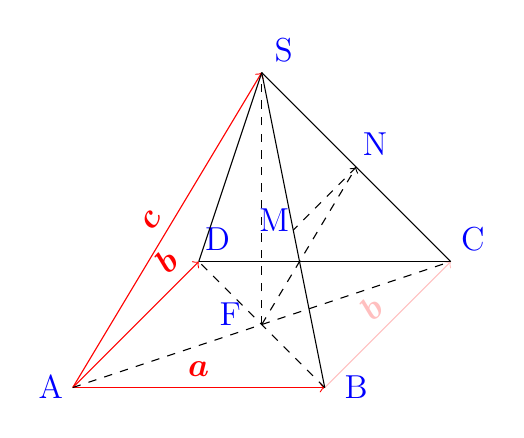
\begin{tikzpicture}[font=\boldmath, scale=0.8]\large
    % Punkte
    \coordinate (A) at (0,0) {};
     \draw[blue] (-0.35,-0.35)   node [above] {A};
    \coordinate (B) at (4,0) {};
    \draw[blue] (4.5,-0.35)   node [above] {B};
    \coordinate (C) at (6,2) {};
    \draw[blue] (6.35,2)   node [above] {C};
    \coordinate (D) at (2,2) {};
    \draw[blue] (2.3,2)   node [above] {D};
    \coordinate (E) at (3,5) {};
    \draw[blue] (3.35,5)   node [above] {S};
    \coordinate (F) at (3,1) {};
    \draw[blue] (2.5,0.8)   node [above] {F};
    \coordinate (G) at (4.5,3.5) {};
    \draw[blue] (4.8,3.5)   node [above] {N};
    \coordinate (H) at (3.5,2.5) {};
    \draw[blue] (3.2,2.3)   node [above] {M};
    \draw[->, red]  (A) -- (B) node[sloped,midway,above] {$\vv{a}$};
    \draw[->,red!25]  (B) -- (C) node[sloped,midway,above] {$\vv{b}$};
    \draw  (C) -- (D) node[] {};
    \draw[->,red]  (A) -- (D) node[sloped,above,very near end] {$\vv{b}$};
   \draw[->,red]  (A) -- (E) node[sloped,midway,above] {$\vv{c}$};
   \draw  (E) -- (B) node[] {};
   \draw  (E) -- (C) node[] {};
   \draw  (E) -- (D) node[] {};
   \draw[dashed]  (A) -- (C) node[] {};
   \draw[dashed]  (B) -- (D) node[] {};
   \draw[dashed]  (F) -- (E) node[] {};
    \draw[dashed]  (G) -- (H) node[] {};
    \draw[->,dashed]  (F) -- (G) node[] {};
\end{tikzpicture} 
    \begin{itemize}
        \item[$\circ$] Vektorkette von $F$ nach $C$ zu $N$.
     \begin{equation*}
            \begin{split}
                \vv{FN} &= \vv{FC} + \vv{CN}\\
                &=\vv{AF} + \dfrac{1}{2} \vv{CS}\\
                &= \dfrac{1}{2} \left(\vv{a} + \vv{b} \right) + \dfrac{1}{2}\left(\vv{c} - \vv{a} -\vv{b}\right)\\
                &=\dfrac{1}{2} \vv{a} + \dfrac{1}{2} \vv{b} + \dfrac{1}{2} \vv{c} - \dfrac{1}{2} \vv{a} -\dfrac{1}{2} \vv{b} \\
                &= \dfrac{1}{2}\vv{c}
            \end{split}
        \end{equation*}
        
    \end{itemize}
   \end{multicols}
   \begin{itemize}
       \item[$\circ$] Daraus folgt, dass der Vektor $\vv{FN}$ parallel und gleichgerichtet zum Vektor $\vv{c}$ aber nur halb so lang ist.
   \end{itemize}
   \begin{enumerate}
    \item[4.] Drücke den Vektor $\vv{MN}$ mithilfe der Vektoren $\vv{a}, \vv{b}$ und $\vv{
    c}$ aus.
    \begin{multicols}{2}
    \begin{itemize}
        \item[$\circ$] Vektorkette von $M$ über $B, C$ zum Punkt $N$.
     \begin{equation*}
            \begin{split}
                \vv{MN} &= - \dfrac{1}{2}\vv{BS} + \vv{BC} + \dfrac{1}{2} \vv{CS}\\
                &= -\dfrac{1}{2} \left( \vv{c} - \vv{a}\right) +\vv{b} + \dfrac{1}{2} \left(\vv{c} - \vv{a} -\vv{b}\right)\\
                &= -\dfrac{1}{2} \vv{c} +\dfrac{1}{2} \vv{a} +\vv{b} + \dfrac{1}{2} \vv{c} - \dfrac{1}{2}\vv{a} -\dfrac{1}{2}\vv{b}\\
                &= \dfrac{1}{2} \vv{b}
            \end{split}
        \end{equation*}  
        \item[$\circ$] Damit folgt, das die Mittellinie $\overline{MN}$ parallel, gleichgerichtet aber nur halb so lang wie der Vektor $\vv{b}$ ist.
    \end{itemize}
    \end{multicols}
\end{enumerate}
\end{bsp}
\section{Der Vektorraum}
\begin{defi}{Der Vektorraum}{}\index{Vektoren!Vektorraum}
    Die Menge aller Vektoren, in der die Gesetze der Addition von Vektoren und deren Multiplikation mit Skalaren gelten, nennt man Vektorraum. Die Basis des Vektorraums setzt sich aus der minimalen Anzahl von Vektoren zusammen die man braucht, um alle anderen Vektoren darstellen zu können. Die Anzahl dieser Vektoren bildet die Dimension des Vektorraums.
\end{defi}
\begin{merke}{Das orthonormale Koordinatensystem}{}\index{Vektoren!orthonormales Koordinatensystem}
    Das zweidimensionale und das dreidimensionale Koordinatensystem der Schulgeometrie ist ein orthonormales Koordinatensystem. Das bedeutet, die Basis besteht aus 2 bzw. 3 Vektoren der Länge eins welche paarweise senkrecht aufeinander stehen. Man bezeichnet diese Vektoren mit $\vv{e}_1, \vv{e}_2, \vv{e}_3$. 
\end{merke}
\begin{b8d}{Die Basisvektoren}{}v\index{Vektoren!Basisvektoren}
Für die Basisvektoren $e_1, e_2$ und $e_3$ gilt folgende Darstellung:\\
$$\vv{e}_1 =\begin{pmatrix} 1 \\ 0 \\0 \end{pmatrix}, 
\vv{e}_2 =\begin{pmatrix} 0 \\ 1 \\0 \end{pmatrix}, 
\vv{e}_3 =\begin{pmatrix} 0 \\ 0 \\1 \end{pmatrix}$$
Mit den Basisvektoren ist man in der Lage, jeden Vektor durch eine Addition der Basisvektoren darzustellen. Diese Darstellung bezeichnet man als Spaltendarstellung der Vektoren. Der Vektor $\vv{a}$ hat damit die Darstellung $\vv{a} = \begin{pmatrix} a_1 \\ a_2 \\a_3 \end{pmatrix} = a_1\cdot \vv{e}_1 + a_2 \cdot \vv{e}_2 + a_3\cdot \vv{e}_3$ mit $a_1, a_2, a_3 \in \mathds{R}$. Die reellen Zahlen $a_i$ nennt man Koordinanten des Vektors $\vv{a}$.  
\end{b8d}
\begin{bem}{Rechnungen mit Vektoren}{}
\begin{itemize}
    \item Addition von Vektoren in der Spaltenschreibweise: Die Vektoren der $\vv{a}$ und $\vv{b}$ werden wie folgt addiert: $$\vv{a} + \vv{b} = \begin{pmatrix} a_1 \\ a_2 \\a_3 \end{pmatrix} + \begin{pmatrix} b_1 \\ b_2 \\b_3 \end{pmatrix} = \begin{pmatrix} a_1 + b_1 \\ a_2 + b_2 \\a_3 + b_3 \end{pmatrix}$$ dabei gilt $a_i, b_i \in \mathds{R}$.
    \item Multiplikation eines Vektors mit einem Skalar: Ein Vektor wird mit einem Skalar wie folgt multipliziert $$\lambda \cdot \vv{a} = \lambda \cdot \begin{pmatrix} a_1 \\ a_2 \\a_3 \end{pmatrix} = \begin{pmatrix} \lambda \cdot a_1 \\ \lambda \cdot a_2 \\\lambda \cdot a_3 \end{pmatrix}$$ mit $\lambda , a_i \in \mathds{R}$.
\end{itemize}
\end{bem}
\begin{satz}{Ortsvektoren}{}\index{Vektoren!Ortsvektor}
Jeder Punkt $P(p_1|p_2|p_3)$ mit $p_i \in \mathds{R}$ des dreidimensionalen Vektorraums lässt sich wie folgt in der Spaltenschreibweise schreiben:
$$\vv{P} = \begin{pmatrix} p_1 \\ p_2 \\p_3 \end{pmatrix}.$$ 
Dieser Vektor repräsentiert genau einen Pfeil der im Urpsrung des Koordinatensystems beginnt und an den Koordinaten des Punktes $P$ endet.\\ 
Diesen Pfeil nennt man Ortsvektor des Punktes $P$.
\end{satz}
\begin{satz}{Verbindungsvektoren}{}
Wird durch den Punkt $A(a_1|a_2|a_3)$ der Anfangspunkt und durch den Punkt $B(b_1|b_2|b_3)$ der Endpunkt eines Vektors festgelegt, so nennt man den dadurch entstehenden Vektor $\vv{AB}$ einen Verbindungsvektor. \\
Die Koordinaten des Verbindungsvektors berechnen sich wie folgt: $$\vv{AB} = \vv{B} -\vv{A} = \begin{pmatrix} b_1 \\ b_2 \\b_3 \end{pmatrix} - \begin{pmatrix} a_1 \\ a_2 \\a_3 \end{pmatrix} = \begin{pmatrix} b_1 - a_1 \\b_2 - a_2 \\b_3 -a_3 \end{pmatrix}$$
für alle $a_i, b_i \in \mathds{R}$.
\end{satz}
\begin{bsp*}{Orts- und Verbindungsvektor}{}
\tdplotsetmaincoords{70}{120}
Gegeben sind die Punkte $P,R$ und $S$ im euklidischen Koordinatensystem. Die Punkte haben folgende Koordinaten: $P(2|3|2), R(3|3|0)$ und $S(0|4|2)$. Damit ergeben sich die die Ortsvektoren:
$$\vv{P} = \begin{pmatrix} 2 \\ 3 \\2 \end{pmatrix}, \vv{R} = \begin{pmatrix} 3 \\ 3 \\0 \end{pmatrix}, \vv{S}=\begin{pmatrix} 0 \\4 \\2 \end{pmatrix}.$$ Die Koordinaten des Verbindungsvektors berechnen sich damit wie folgt:
$$\vv{RS} = \vv{S} - \vv{R} = \begin{pmatrix} 0 \\4 \\2 \end{pmatrix} - \begin{pmatrix} 3 \\ 3 \\0 \end{pmatrix}=  \begin{pmatrix} -3 \\ 1 \\2 \end{pmatrix}$$
\begin{tikzpicture}[scale=2, tdplot_main_coords, axis/.style={-> }, 
vector/.style={-stealth,red}, 
vector guide/.style={dashed,red}]
% -- remove these 3 lines if no axis is preferred
\draw[axis] (0, 0, 0) -- (5, 0, 0) node [left] {$x_1$};
\draw[axis] (0, 0, 0) -- (0, 5, 0) node [above] {$x_2$};
\draw[axis] (0, 0, 0) -- (0, 0, 2) node [above] {$x_3$};
% define points
\coordinate  (d1) at (0,0,0){};
\coordinate  (d2) at (4,0,0){};
\coordinate  (d3) at (2,3,2){};
\coordinate  (d4) at (0,4,2){};
\coordinate  (d5) at (3,3,0){};
\draw[blue] (2,3,2)   node [above] {$P$};
\draw[vector] (d1) -- (d3);
 %\draw (0,0,0) -- ++(-2.5pt,-2.5pt) -- ++(5pt,5pt) ++(-5pt,0pt) -- ++(5pt,-5pt);
  %\draw (2,3,2) -- ++(-2.5pt,-2.5pt) -- ++(5pt,5pt) ++(-5pt,0pt) -- ++(5pt,-5pt);
\draw[vector] (d5) -- (d4);
\draw[blue] (3,3,0)   node [above] {$R$};
\draw[blue] (0,4,2)   node [above] {$S$};
\draw[vector, blue, dashed] (d1) -- (d4);
\draw[vector, blue, dashed] (d1) -- (d5);
\draw[blue] (1.5,1.5,0)   node [above] {$\vv{R}$};
\draw[blue] (0,2,0.6)   node [above] {$\vv{S}$};
\draw[blue] (0,1,0.6)   node [above] {$\vv{P}$};
\end{tikzpicture}
\end{bsp*}
Durch die Verwendung von Koordinaten in der Vektorgeometrie ist es möglich spezielle Punkte relativ einfach zu berechnen. So ist es jetzt möglich, dass man zum Beispiel eine den Mittelpunkt einer Strecke bestimmt oder eine Strecke zu verdoppeln.
\begin{b8d*}{Eigenschaften einer Strecke}{}
Für den Ortsvektor $\vv{M}$ des Mittelpunktes der Strecke $\overline{AB}$ gilt: $$\vv{M} = \dfrac{1}{2}\left(\vv{A} + \vv{B}\right).$$
Die Strecke $\overline{AB}$ lässt sich so, einfach in beliebig viele Teile einteilen. 
\end{b8d*}
\begin{bsp*}{Teilungen einer Strecke}{}
Die Punkte $A$ und $B$ mit den Koordinaten $\vv{A} = \begin{pmatrix} 4 \\0 \\2 \end{pmatrix}$ und $\vv{B}= \begin{pmatrix} -2 \\3 \\5 \end{pmatrix}$ bestimmen eine Strecke $\overline{AB}$. Um die Strecke in vier gleich große Teile einzuteilen bestimmt man als erstes den Mittelpunkt. $$\vv{M_1}=\dfrac{1}{2}\left(\vv{A} + \vv{B}\right) = \dfrac{1}{2}\left( \begin{pmatrix} 4 \\0 \\2 \end{pmatrix} +  \begin{pmatrix} -2 \\3 \\5 \end{pmatrix} \right)= \dfrac{1}{2}\begin{pmatrix} 2 \\3 \\7 \end{pmatrix} = \begin{pmatrix} 1 \\1,5 \\3,5 \end{pmatrix}. $$ 
Anschließend werden die Mittelpunkte der Strecken $\overline{AM_1}$ und $\overline{M_1B}$ berechnet.
$$\vv{M_2} = \dfrac{1}{2}\left(\vv{A} + \vv{M_1}\right) =  \dfrac{1}{2} \left( \begin{pmatrix} 4 \\0 \\2 \end{pmatrix}  + \begin{pmatrix} 1 \\1,5 \\3,5 \end{pmatrix} \right) = \dfrac{1}{2} \begin{pmatrix} 5 \\1,5 \\5,5 \end{pmatrix} = \begin{pmatrix} 2,5 \\0,75 \\2,75 \end{pmatrix}$$
$$\vv{M_3} = \dfrac{1}{2}\left(\vv{M_1} + \vv{B}\right) =  \dfrac{1}{2} \left( \begin{pmatrix} 1 \\1,5 \\3,5 \end{pmatrix} +   \begin{pmatrix} -2 \\3 \\5 \end{pmatrix} \right) = \dfrac{1}{2} \begin{pmatrix} -1 \\4,5 \\8,5 \end{pmatrix} =  \begin{pmatrix} -0,5 \\2,25 \\4,25 \end{pmatrix}$$
Durch die Berechnung der Punkte ergeben sich 4 gleich große Teilstücke. \\
Die Strecken $\overline{AM_2}, \ \overline{M_2M_1}, \ \overline{M_1M_3}$ und $\overline{M_3B}.$
\begin{center}
 
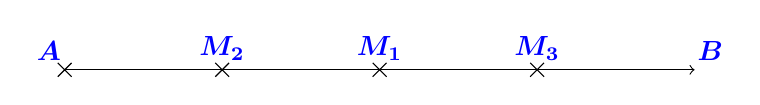
\begin{tikzpicture}[font=\boldmath]
    % Punkte
    \coordinate (C) at (1,3) {};
    \coordinate (D) at (9,3) {};   
    
    \draw[->]  (C) -- (D) node[sloped,midway,above] {};
    \draw[blue] (0.8,3)   node [above] {$A$};
    \draw (1, 3) -- ++(-2.5pt,-2.5pt) -- ++(5pt,5pt) ++(-5pt,0pt) -- ++(5pt,-5pt);
    \draw[blue] (9.2,3)   node [above] {$B$};
       % \draw (9, 3) -- ++(-2.5pt,-2.5pt) -- ++(5pt,5pt) ++(-5pt,0pt) -- ++(5pt,-5pt);
 \draw[blue] (5,3)   node [above] {$M_1$};
        \draw (5, 3) -- ++(-2.5pt,-2.5pt) -- ++(5pt,5pt) ++(-5pt,0pt) -- ++(5pt,-5pt);
 \draw[blue] (3,3)   node [above] {$M_2$};
        \draw (3, 3) -- ++(-2.5pt,-2.5pt) -- ++(5pt,5pt) ++(-5pt,0pt) -- ++(5pt,-5pt);
 \draw[blue] (7,3)   node [above] {$M_3$};
        \draw (7, 3) -- ++(-2.5pt,-2.5pt) -- ++(5pt,5pt) ++(-5pt,0pt) -- ++(5pt,-5pt);     
\end{tikzpicture} 
\end{center}
\end{bsp*}
